\documentclass[english,hidelinks, 11 pt, class=report,crop=false]{standalone}
\usepackage[T1]{fontenc}
%\usepackage[utf8]{inputenc}
\usepackage{lmodern} % load a font with all the characters
\usepackage{geometry}
\geometry{verbose,paperwidth=16.1 cm, paperheight=24 cm, inner=2.3cm, outer=1.8 cm, bmargin=2cm, tmargin=1.8cm}
\setlength{\parindent}{0bp}
\usepackage{import}
\usepackage[subpreambles=false]{standalone}
\usepackage{amsmath}
\usepackage{amssymb}
\usepackage{esint}
\usepackage{babel}
\usepackage{tabu}
\makeatother
\makeatletter

\usepackage{titlesec}
\usepackage{ragged2e}
\RaggedRight
\raggedbottom
\frenchspacing

\usepackage{graphicx}
\usepackage{float}
\usepackage{subfig}
\usepackage{placeins}
\usepackage{cancel}
\usepackage{framed}
\usepackage{wrapfig}
\usepackage[subfigure]{tocloft}
\usepackage[font=footnotesize,labelfont=sl]{caption} % Figure caption
\usepackage{bm}
\usepackage[dvipsnames, table]{xcolor}
\definecolor{shadecolor}{rgb}{0.105469, 0.613281, 1}
\colorlet{shadecolor}{Emerald!15} 
\usepackage{icomma}
\makeatother
\usepackage[many]{tcolorbox}
\usepackage{multicol}
\usepackage{stackengine}

\usepackage{esvect} %For vectors with capital letters

% For tabular
\usepackage{array}
\usepackage{multirow}
\usepackage{longtable} %breakable table

% Ligningsreferanser
\usepackage{mathtools} % for mathclap
%\mathtoolsset{showonlyrefs}

% sections without numbering in toc
\newcommand\tsec[1]{\phantomsection \addcontentsline{toc}{section}{#1}
	\section*{#1}}

% index
\usepackage{imakeidx}
\makeindex[title=Indeks]

%Footnote:
\usepackage[bottom, hang, flushmargin]{footmisc}
\usepackage{perpage} 
\MakePerPage{footnote}
\addtolength{\footnotesep}{2mm}
\renewcommand{\thefootnote}{\arabic{footnote}}
\renewcommand\footnoterule{\rule{\linewidth}{0.4pt}}
\renewcommand{\thempfootnote}{\arabic{mpfootnote}}

%colors
\definecolor{c1}{cmyk}{0,0.5,1,0}
\definecolor{c2}{cmyk}{1,0.25,1,0}
\definecolor{n3}{cmyk}{1,0.,1,0}
\definecolor{neg}{cmyk}{1,0.,0.,0}


\newcommand{\nreq}[1]{
\begin{equation}
	#1
\end{equation}
}


% Equation comments
\newcommand{\cm}[1]{\llap{\color{blue} #1}}


\usepackage[inline]{enumitem}
\newcounter{rg}
\numberwithin{rg}{chapter}


\newcommand{\reg}[2][]{\begin{tcolorbox}[boxrule=0.3 mm,arc=0mm,colback=blue!3] {\refstepcounter{rg}\phantomsection \large \textbf{\therg \;#1} \vspace{5 pt}}\newline #2  \end{tcolorbox}\vspace{-5pt}}
\newcommand{\regdef}[2][]{\begin{tcolorbox}[boxrule=0.3 mm,arc=0mm,colback=blue!3] {\refstepcounter{rg}\phantomsection \large \textbf{\therg \;#1} \vspace{5 pt}}\newline #2  \end{tcolorbox}\vspace{-5pt}}
\newcommand{\words}[1]{\begin{tcolorbox}[boxrule=0.3 mm,arc=0mm,colback=teal!3] #1  \end{tcolorbox}\vspace{-5pt}}

\newcommand\alg[1]{\begin{align*} #1 \end{align*}}

\newcommand\eks[2][]{\begin{tcolorbox}[boxrule=0.3 mm,arc=0mm,enhanced jigsaw,breakable,colback=green!3] {\large \textbf{\ekstitle #1} \vspace{5 pt}\\} #2 \end{tcolorbox}\vspace{-5pt} }

\newcommand{\st}[1]{\begin{tcolorbox}[boxrule=0.0 mm,arc=0mm,enhanced jigsaw,breakable,colback=yellow!12]{ #1} \end{tcolorbox}}

\newcommand{\spr}[1]{\begin{tcolorbox}[boxrule=0.3 mm,arc=0mm,enhanced jigsaw,breakable,colback=yellow!7] {\large \textbf{\sprtitle} \vspace{5 pt}\\} #1 \end{tcolorbox}\vspace{-5pt} }

\newcommand{\sym}[1]{\colorbox{blue!15}{#1}}

\newcommand{\info}[2]{\begin{tcolorbox}[boxrule=0.3 mm,arc=0mm,enhanced jigsaw,breakable,colback=cyan!6] {\large \textbf{#1} \vspace{5 pt}\\} #2 \end{tcolorbox}\vspace{-5pt} }

\newcommand\algv[1]{\vspace{-11 pt}\begin{align*} #1 \end{align*}}

\newcommand{\regv}{\vspace{5pt}}
\newcommand{\mer}{\textsl{\note}: }
\newcommand{\mers}[1]{{\footnotesize \mer #1}}
\newcommand\vsk{\vspace{11pt}}
\newcommand{\tbs}{\vspace{5pt}}
\newcommand\vs{\vspace{-11pt}}
\newcommand\vsb{\vspace{-16pt}}
\newcommand\br{\\[5 pt]}
\newcommand{\figp}[1]{../fig/#1}
\newcommand\algvv[1]{\vs\vs\begin{align*} #1 \end{align*}}
\newcommand{\y}[1]{$ {#1} $}
\newcommand{\os}{\\[5 pt]}
\newcommand{\prbxl}[2]{
\parbox[l][][l]{#1\linewidth}{#2
	}}
\newcommand{\prbxr}[2]{\parbox[r][][l]{#1\linewidth}{
		\setlength{\abovedisplayskip}{5pt}
		\setlength{\belowdisplayskip}{5pt}	
		\setlength{\abovedisplayshortskip}{0pt}
		\setlength{\belowdisplayshortskip}{0pt} 
		\begin{shaded}
			\footnotesize	#2 \end{shaded}}}
\newcommand{\fgbxr}[2]{
	\parbox[r][][l]{#1\linewidth}{#2
}}		

\renewcommand{\cfttoctitlefont}{\Large\bfseries}
\setlength{\cftaftertoctitleskip}{0 pt}
\setlength{\cftbeforetoctitleskip}{0 pt}

\newcommand{\bs}{\\[3pt]}
\newcommand{\vn}{\\[6pt]}
\newcommand{\fig}[1]{\begin{figure}[H]
		\centering
		\includegraphics[]{\figp{#1}}
\end{figure}}

\newcommand{\figc}[2]{\begin{figure}
		\centering
		\includegraphics[]{\figp{#1}}
		\caption{#2}
\end{figure}}
\newcommand{\arc}[1]{{
		\setbox9=\hbox{#1}%
		\ooalign{\resizebox{\wd9}{\height}{\texttoptiebar{\phantom{A}}}\cr\textit{#1}}}}

\newcommand{\sectionbreak}{\clearpage} % New page on each section

\newcommand{\nn}[1]{
\begin{equation*}
	#1
\end{equation*}
}

\newcommand{\enh}[1]{\,\textrm{#1}}

%asin, atan, acos
\DeclareMathOperator{\atan}{atan}
\DeclareMathOperator{\acos}{acos}
\DeclareMathOperator{\asin}{asin}

% Comments % old cm, ggb cm is new
%\newcommand{\cm}[1]{\llap{\color{blue} #1}}

%%%

\newcommand\fork[2]{\begin{tcolorbox}[boxrule=0.3 mm,arc=0mm,enhanced jigsaw,breakable,colback=yellow!7] {\large \textbf{#1 (\expl)} \vspace{5 pt}\\} #2 \end{tcolorbox}\vspace{-5pt} }
 
%colors
\newcommand{\colr}[1]{{\color{red} #1}}
\newcommand{\colb}[1]{{\color{blue} #1}}
\newcommand{\colo}[1]{{\color{orange} #1}}
\newcommand{\colc}[1]{{\color{cyan} #1}}
\definecolor{projectgreen}{cmyk}{100,0,100,0}
\newcommand{\colg}[1]{{\color{projectgreen} #1}}

% Methods
\newcommand{\metode}[2]{
	\textsl{#1} \\[-8pt]
	\rule{#2}{0.75pt}
}

%Opg
\newcommand{\abc}[1]{
	\begin{enumerate}[label=\alph*),leftmargin=18pt]
		#1
	\end{enumerate}
}
\newcommand{\abcs}[2]{
	\begin{enumerate}[label=\alph*),start=#1,leftmargin=18pt]
		#2
	\end{enumerate}
}
\newcommand{\abcn}[1]{
	\begin{enumerate}[label=\arabic*),leftmargin=18pt]
		#1
	\end{enumerate}
}
\newcommand{\abch}[1]{
	\hspace{-2pt}	\begin{enumerate*}[label=\alph*), itemjoin=\hspace{1cm}]
		#1
	\end{enumerate*}
}
\newcommand{\abchs}[2]{
	\hspace{-2pt}	\begin{enumerate*}[label=\alph*), itemjoin=\hspace{1cm}, start=#1]
		#2
	\end{enumerate*}
}

% Exercises


\newcounter{opg}
\numberwithin{opg}{section}

\newcounter{grub}
\numberwithin{opg}{section}
\newcommand{\op}[1]{\vspace{15pt} \refstepcounter{opg}\large \textbf{\color{blue}\theopg} \vspace{2 pt} \label{#1} \\}
\newcommand{\eksop}[2]{\vspace{15pt} \refstepcounter{opg}\large \textbf{\color{blue}\theopg} (#1) \vspace{2 pt} \label{#2} \\}

\newcommand{\nes}{\stepcounter{section}
	\setcounter{opg}{0}}
\newcommand{\opr}[1]{\vspace{3pt}\textbf{\ref{#1}}}
\newcommand{\oeks}[1]{\begin{tcolorbox}[boxrule=0.3 mm,arc=0mm,colback=white]
		\textit{\ekstitle: } #1	  
\end{tcolorbox}}
\newcommand\opgeks[2][]{\begin{tcolorbox}[boxrule=0.1 mm,arc=0mm,enhanced jigsaw,breakable,colback=white] {\footnotesize \textbf{\ekstitle #1} \\} \footnotesize #2 \end{tcolorbox}\vspace{-5pt} }


% tag exercises
\newcommand{\tagop}[1]{ 
{\small \color{Gray} #1} \os
}

% License
\newcommand{\lic}{
This book is part of the \net{https://sindrsh.github.io/openmathbooks/}{OpenMathBooks} project. OpenMathBooks © 2022 by Sindre Sogge Heggen is licensed under CC BY-NC-SA 4.0. To view a copy of this license, visit \net{http://creativecommons.org/licenses/by-nc-sa/4.0/}{http://creativecommons.org/licenses/by-nc-sa/4.0/}}

%referances
\newcommand{\net}[2]{{\color{blue}\href{#1}{#2}}}
\newcommand{\hrs}[2]{\hyperref[#1]{\color{blue}#2 \ref*{#1}}}
\newcommand{\refunnbr}[2]{\hyperref[#1]{\color{blue}#2}}


\newcommand{\openmath}{\net{https://sindrsh.github.io/openmathbooks/}{OpenMathBooks}}
\newcommand{\am}{\net{https://sindrsh.github.io/FirstPrinciplesOfMath/}{AM1}}
\newcommand{\mb}{\net{https://sindrsh.github.io/FirstPrinciplesOfMath/}{MB}}
\newcommand{\tmen}{\net{https://sindrsh.github.io/FirstPrinciplesOfMath/}{TM1}}
\newcommand{\tmto}{\net{https://sindrsh.github.io/FirstPrinciplesOfMath/}{TM2}}
\newcommand{\amto}{\net{https://sindrsh.github.io/FirstPrinciplesOfMath/}{AM2}}
\newcommand{\eksbm}{
\footnotesize
Dette er opppgaver som har blitt gitt ved sentralt utformet eksamen i Norge. Oppgavene er laget av Utdanningsdirektoratet. Forkortelser i parantes viser til følgende:
\begin{center}
	\begin{tabular}{c|c}
		E & Eksempeloppgave \\
		V/H & Eksamen fra vårsemesteret/høstsemesteret\\
		G/1P/1T/R1/R2 & Fag  \\
		XX & År 20XX \\
		D1/D2 & Del 1/Del 2
	\end{tabular}
\end{center}
Tekst og innhold kan her være noe endret i forhold til originalen.
}

%Excel og GGB:

\newcommand{\g}[1]{\begin{center} {\tt #1} \end{center}}
\newcommand{\gv}[1]{\begin{center} \vspace{-11 pt} {\tt #1}  \end{center}}
\newcommand{\cmds}[2]{{\tt #1}\\
	#2}

% outline word
\newcommand{\outl}[1]{{\boldmath \color{teal}\textbf{#1}}}
%line to seperate examples
\newcommand{\linje}{\rule{\linewidth}{1pt} }


%Vedlegg
\newcounter{vedl}
\newcounter{vedleq}
\renewcommand\thevedl{\Alph{vedl}}	
\newcommand{\nreqvd}{\refstepcounter{vedleq}\tag{\thevedl \thevedleq}}

%%% Writing code

\usepackage{listings}


\definecolor{codegreen}{rgb}{0,0.6,0}
\definecolor{codegray}{rgb}{0.5,0.5,0.5}
\definecolor{codepurple}{rgb}{0.58,0,0.82}
\definecolor{backcolour}{rgb}{0.95,0.95,0.92}

\newcommand{\pymet}[1]{{\ttfamily\color{magenta} #1}}
\newcommand{\pytype}[1]{{\ttfamily\color{codepurple} #1}}

\lstdefinestyle{mystyle}{
	backgroundcolor=\color{backcolour},   
	commentstyle=\color{codegreen},
	keywordstyle=\color{magenta},
	numberstyle=\tiny\color{codegray},
	stringstyle=\color{codepurple},
	basicstyle=\ttfamily\footnotesize,
	breakatwhitespace=false,         
	breaklines=true,                 
	captionpos=b,                    
	keepspaces=true,                 
	numbers=left,                    
	numbersep=5pt,                  
	showspaces=false,                
	showstringspaces=false,
	showtabs=false,                  
	tabsize=2,
	inputencoding=utf8,
	extendedchars=true,
	literate= {
		{å}{{\aa}}1 
		{æ}{{\ae}}1 
		{ø}{{\o}}1
	}
}

\lstset{style=mystyle}

\newcommand{\python}[1]{
\begin{tcolorbox}[boxrule=0.3 mm,arc=0mm,colback=white]
\lstinputlisting[language=Python]{#1}
\end{tcolorbox}}
\newcommand{\pythonut}[2]{
\begin{tcolorbox}[boxrule=0.3 mm,arc=0mm,colback=white]
\small 
%\textbf{Kode}
\lstinputlisting[language=Python]{#1}	
\vspace{11pt}
\textbf{Utdata} \\ \ttfamily
#2
\end{tcolorbox}}
%%%

%page number
%\usepackage{fancyhdr}
%\pagestyle{fancy}
%\fancyhf{}
%\renewcommand{\headrule}{}
%\fancyhead[RO, LE]{\thepage}

\usepackage{datetime2}
%%\usepackage{sansmathfonts} for dyslexia-friendly math
\usepackage[]{hyperref}


% note
\newcommand{\note}{Note}
\newcommand{\notesm}[1]{{\footnotesize \textsl{\note:} #1}}
\newcommand{\selos}{See the solutions manual.}

\newcommand{\texandasy}{The text is written in \LaTeX\ and the figures are made with the aid of Asymptote.}

\newcommand{\rknut}{Calculate.}
\newcommand\sv{\vsk \textbf{Answer} \vspace{4 pt}\\}
\newcommand{\ekstitle}{Example }
\newcommand{\sprtitle}{The language box}
\newcommand{\expl}{explanation}

% answers
\newcommand{\mulansw}{\notesm{Multiple possible answers.}}	
\newcommand{\faskap}{Chapter}

% exercises
\newcommand{\opgt}{\newpage \phantomsection \addcontentsline{toc}{section}{Exercises} \section*{Exercises for Chapter \thechapter}\vs \setcounter{section}{1}}

\newcommand{\grubop}[1]{\vspace{15pt} \refstepcounter{grub}\large \textbf{\color{blue} Ponder \thegrub} \vspace{2 pt} \label{#1} \\}
\newcommand{\grubr}[1]{\vspace{3pt}\textbf{Ponder \ref{#1}}}


% references
\newcommand{\reftab}[1]{\hrs{#1}{Table}}
\newcommand{\rref}[1]{\hrs{#1}{Rule}}
\newcommand{\dref}[1]{\hrs{#1}{Definition}}
\newcommand{\refkap}[1]{\hrs{#1}{Chapter}}
\newcommand{\refsec}[1]{\hrs{#1}{Section}}
\newcommand{\refdsec}[1]{\hrs{#1}{Subsection}}
\newcommand{\refved}[1]{\hrs{#1}{Appendix}}
\newcommand{\eksref}[1]{\textsl{#1}}
\newcommand\fref[2][]{\hyperref[#2]{\textsl{Figure \ref*{#2}#1}}}
\newcommand{\refop}[1]{{\color{blue}Exercise \ref{#1}}}
\newcommand{\refops}[1]{{\color{blue}Exercise \ref{#1}}}

%%% SECTION HEADLINES %%%

% Our numbers
\newcommand{\likteikn}{The equal sign}
\newcommand{\talsifverd}{Numbers, digits and values}
\newcommand{\koordsys}{Coordinate systems}

% Calculations
\newcommand{\adi}{Addition}
\newcommand{\sub}{Subtraction}
\newcommand{\gong}{Multiplication}
\newcommand{\del}{Division}

%Factorization and order of operations
\newcommand{\fak}{Factorization}
\newcommand{\rrek}{Order of operations}

%Fractions
\newcommand{\brgrpr}{Introduction}
\newcommand{\brvu}{Values, expanding and simplifying}
\newcommand{\bradsub}{Addition and subtraction}
\newcommand{\brgngheil}{Fractions multiplied by integers}
\newcommand{\brdelheil}{Fractions divided by integers}
\newcommand{\brgngbr}{Fractions multiplied by fractions}
\newcommand{\brkans}{Cancelation of fractions}
\newcommand{\brdelmbr}{Division by fractions}
\newcommand{\Rasjtal}{Rational numbers}

%Negative numbers
\newcommand{\negintro}{Introduction}
\newcommand{\negrekn}{The elementary operations}
\newcommand{\negmeng}{Negative numbers as amounts}

%Calculation methods
\newcommand{\delmedtihundre}{Deling med 10, 100, 1\,000 osv.}

% Geometry 1
\newcommand{\omgr}{Terms}
\newcommand{\eignsk}{Attributes of triangles and quadrilaterals}
\newcommand{\omkr}{Perimeter}
\newcommand{\area}{Area}

%Algebra 
\newcommand{\algintro}{Introduction}
\newcommand{\pot}{Powers}
\newcommand{\irrasj}{Irrational numbers}

%Equations
\newcommand{\ligintro}{Introduction}
\newcommand{\liglos}{Solving with the elementary operations}
\newcommand{\ligloso}{Solving with elementary operations summarized}

%Functions
\newcommand{\fintro}{Introduction}
\newcommand{\lingraf}{Linear functions and graphs}

%Geometry 2
\newcommand{\geoform}{Formulas of area and perimeter}
\newcommand{\kongogsim}{Congruent and similar triangles}
\newcommand{\geofork}{Explanations}

% Names of rules
\newcommand{\adkom}{Addition is commutative}
\newcommand{\gangkom}{Multiplication is commutative}
\newcommand{\brdef}{Fractions as rewriting of division}
\newcommand{\brtbr}{Fractions multiplied by fractions}
\newcommand{\delmbr}{Fractions divided by fractions}
\newcommand{\gangpar}{Distributive law}
\newcommand{\gangparsam}{Paranthesis multiplied together}
\newcommand{\gangmnegto}{Multiplication by negative numbers I}
\newcommand{\gangmnegtre}{Multiplication by negative numbers II}
\newcommand{\konsttre}{Unique construction of triangles}
\newcommand{\kongtre}{Congruent triangles}
\newcommand{\topv}{Vertical angles}
\newcommand{\trisum}{The sum of angles in a triangle}
\newcommand{\firsum}{The sum of angles in a quadrilateral}
\newcommand{\potgang}{Multiplication by powers}
\newcommand{\potdivpot}{Division by powers}
\newcommand{\potanull}{The special case of \boldmath $a^0$}
\newcommand{\potneg}{Powers with negative exponents}
\newcommand{\potbr}{Fractions as base}
\newcommand{\faktgr}{Factors as base}
\newcommand{\potsomgrunn}{Powers as base}
\newcommand{\arsirk}{The area of a circle}
\newcommand{\artrap}{The area of a trapezoid}
\newcommand{\arpar}{The area of a parallelogram}
\newcommand{\pyt}{Pythagoras's theorem}
\newcommand{\forform}{Ratios in similar triangles}
\newcommand{\vilkform}{Terms of similar triangles}
\newcommand{\omkrsirk}{The perimeter of a circle (and the value of $ \bm \pi $)}
\newcommand{\artri}{The area of a triangle}
\newcommand{\arrekt}{The area of a rectangle}
\newcommand{\liknflyt}{Moving terms across the equal sign}
\newcommand{\funklin}{Linear functions}


\begin{document}
\section{Spreadsheets}

\textit{In this book, we base our discussions on Microsoft's software, Excel. There are other good spreadsheets available in the market, such as Google Sheets and Libre Office Calc. These three mentioned spreadsheets are very similar in design and in the functions they offer.}

\subsection{Introduction}

When you open a spreadsheet, you'll see a table where \textit{rows} are numbered with numbers (1, 2, 3 etc.), while \textit{columns} are indexed with letters (A, B, C etc.). How the rows and columns are used is crucial for understanding Excel. In the figure below, we have highlighted what we call \textit{cell B\textsl{3}}. This is the cell where \textsl{row 3 and column B intersect}. (Also, notice that B3 is highlighted in the top left of the figure).

\begin{figure}[H]
	\centering
	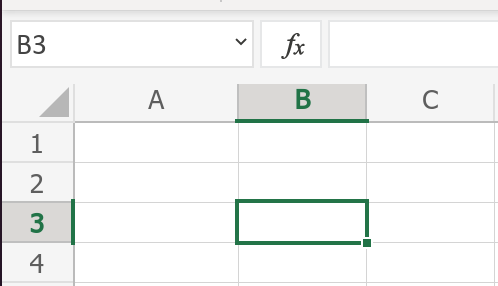
\includegraphics[scale=0.25]{figs/B3}
\end{figure}
In each cell, we can input both numbers and text. Let's say Ole has a job with an hourly wage of 250\,kr, and he works 7 hours a week. We can input this information into Excel as shown:
\begin{figure}[H]
	\centering
	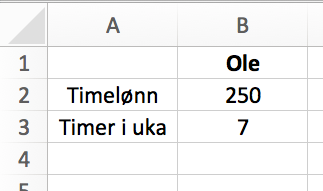
\includegraphics[scale=0.35]{figs/ex2}
\end{figure}
\subsection{Calculations}
Now, we want to determine Ole's weekly wage.
The weekly wage is given by the formula
\[ \text{weekly wage}={\text{hourly wage}\cdot \text{hours per week}} \]
To perform a calculation in a spreadsheet, you start by typing {\tt{=}} in the cell. In cell B4, we find Ole's weekly wage by typing {\tt=250$ ^* $7}.
\begin{figure}[H]
	\centering
	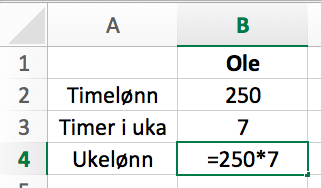
\includegraphics[scale=0.3]{figs/ex3}\qquad
	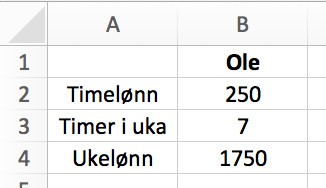
\includegraphics[scale=0.3]{figs/ex4}
\end{figure}
When we press the enter key, the result, 1750, is displayed in the cell. If you want to see the formula we used, you can double click on the cell, or look at the \textit{input field} (top right in the figure below).
\begin{figure}[H]
	\centering
	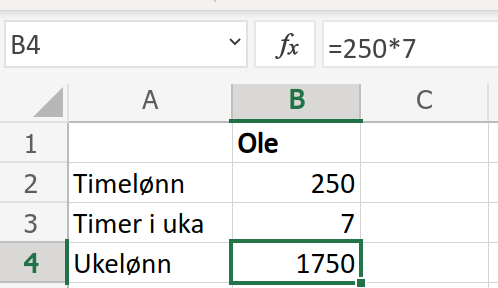
\includegraphics[scale=0.25]{figs/intast}
\end{figure}
\textsl{Note:} The input field can also be used to input numbers and text in the cell.

\subsection{Cell References}
Perhaps Excel's most essential feature is \textit{cell references}. In short, this means that we use cells instead of numbers when making calculations. In the previous section, we calculated Ole's wage by multiplying 250 (hourly wage) by 7 (hours per week). By using cell references, we could have done this instead:

The number corresponding to the hourly wage (250) is in cell B2, while the number corresponding to hours (35) is in cell B3. To multiply the numbers in these cells, we can type {\tt =B2$ ^* $B3}: 

\begin{figure}[H]
	\centering
	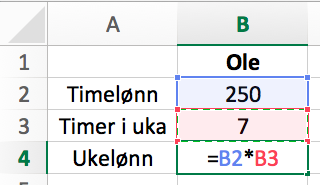
\includegraphics[scale=0.3]{figs/ex5}\qquad
	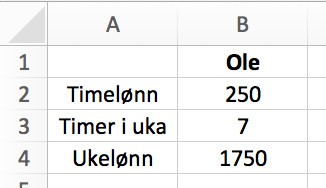
\includegraphics[scale=0.3]{figs/ex4}
\end{figure}
One advantage of using cell references is that it becomes much easier to correct mistakes that have been made. Say, for instance, it should have been 300 instead of 250 in B3. If we change B3, the result in B4 will adjust accordingly:
\begin{figure}[H]
	\centering
	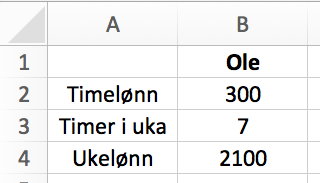
\includegraphics[scale=0.3]{figs/ex6}
\end{figure}
\textsl{Note:} You can also click on the cells you want to use in your formulas, as shown \net{https://drive.google.com/open?id=1S43og4XFAiYyZeFh7tGClBYXoPSv2i0R}{here}.

\subsection{Copying and Locking Cells}
Copying cells is a method that prevents you from writing the same formulas over and over again. We now want to create a sheet suitable for the following information:
\begin{itemize}
	\item The hourly wages for Ole, Dole, and Doffen are 300\,kr, 200\,kr, and 500\,kr, respectively.
	\item All three work 7 days a week.
	\item We want to calculate the total hours they work and their total weekly wages.
\end{itemize}

We start by setting up this spreadsheet:
\begin{figure}[H]
	\centering
	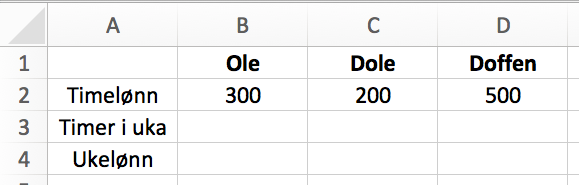
\includegraphics[scale=0.3]{figs/ex7}\qquad
\end{figure}
Here, we have only filled in the information that is \textit{unique} for Ole, Dole, and Doffen, precisely because the other cells either contain the same numbers or use the same calculation method. For cells that are not unique, we should use the copying features, as shown in this \net{??}{video}. Here is a brief description of what is done:
\begin{enumerate}
	\item Since all three work 7 hours, we type {\tt 7} in cell B4. Then, we copy by clicking the mouse pointer right at the bottom right corner of B4 and drag \textsl{across} to C2 and D2.
	\item Since the calculation method for weekly wages is the same for all three, we type it (with cell references) in B4, and copy it \textsl{across} to cell C4 and D4.
	\item The calculation method for the sum of hours and the sum of weekly wages is also the same; hence, we type it in cell E3 and copy it \textsl{down} to E4.
\end{enumerate}
The result is:
\begin{figure}[H]
	\centering
	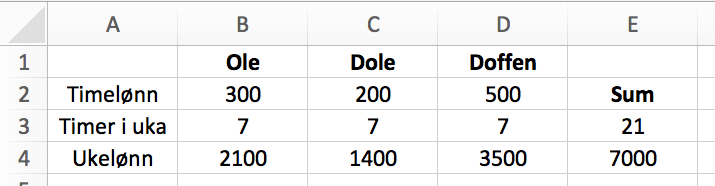
\includegraphics[scale=0.3]{figs/ex8}\\[5pt]
	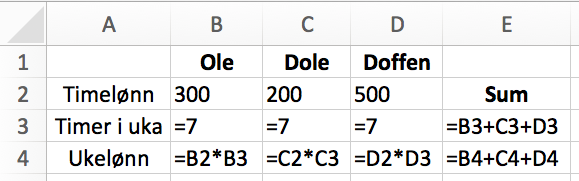
\includegraphics[scale=0.3]{figs/ex15}
\end{figure}
From what we've seen in the \net{https://drive.google.com/open?id=1FgpfKxFzfrc18sIoy3B1MBfEguvzSzVJ}{video} and the figures above, we can take away two general rules:
\begin{enumerate}
	\item Every time you copy a formula one cell \textsl{across}, the columns in the formula will increase by one letter in the alphabet. (A becomes B, B becomes C, etc.)
	\item Every time you copy a formula one cell \textsl{down}, the rows in the formula will increase by 1 (1 becomes 2, 2 becomes 3, etc.).
\end{enumerate}

\textbf{Locking of cells}\\[2pt]
When copying cells, it's essential to watch out for cells you want to use in all copies, because these cells must be \textit{locked}. Let's say for instance that Huey, Dewey, and Louie all work 48 weeks a year. To find their annual salary, we must multiply the weekly wage of each of them by 48. \vsk

Again, we note that the calculation method to find the annual salary is the same for all three. However, if we use cell B8 in a formula and copy as we have done so far, the letter B will change in the formulas. To avoid this, we write {\tt \$} in front of {\tt B} in the formula $ - $ this ensures that the column letter doesn't change, even if we copy the formula. This is shown in this \net{https://drive.google.com/open?id=1bPz2NYZEB3iWyCMQQYTpgms8LsTepY_G}{video}, and the result looks like this:
\begin{figure}[H]
	\centering
	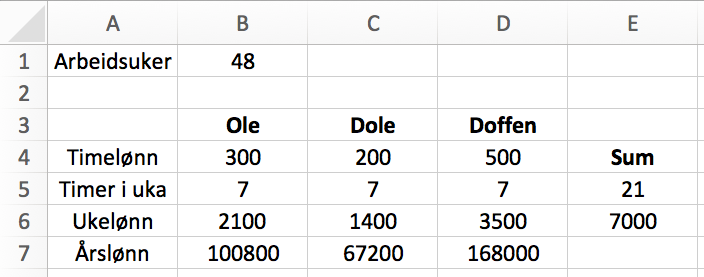
\includegraphics[scale=0.3]{figs/ex12}\\[5pt]
	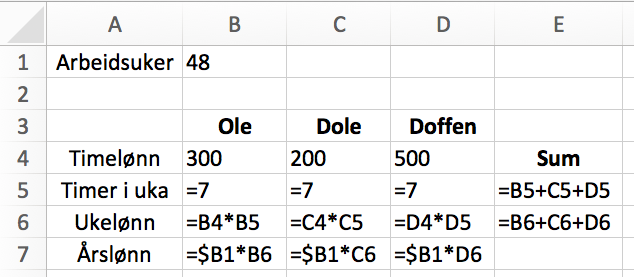
\includegraphics[scale=0.3]{figs/ex13}
\end{figure}
To lock a cell \textsl{downwards}, we must place the dollar sign in front of the row number, for instance {\tt{B\$1}}.
\subsection{Other useful functions}
\st{
	\textbf{Videos}
	\begin{itemize}
		\item \net{https://drive.google.com/file/d/1o7DuDB4yd47kfJWRGXn5Gp3yQbskZiVC/view?usp=sharing}{Sum across and sum down}	
		\item \net{https://drive.google.com/file/d/1RoEAzBYq0bkf1T-W_iWfKW4cc4inlRtb/view?usp=sharing}{Adjust column width}
		\item \net{https://drive.google.com/file/d/1ZiRWW8CwNgSRvjng6JFxKhFZ5HmWLSXM/view?usp=sharing}{Insert row}
		\item \net{https://drive.google.com/file/d/1iuDPTMvDeA73HCjhXIp9nhdMdWou2qhI/view?usp=sharing}{Formula view}
		\item \net{https://drive.google.com/file/d/1EdnLdzkRKL_L7ipeEtNc8wyDlS-f2h9X/view?usp=sharing}{Convert to percentage}
		\item \net{https://drive.google.com/file/d/1ueFQnTNYIGEH6lMxXc0o_PWcl7204YVZ/view?usp=sharing}{Change the number of decimals}
		\item \net{https://drive.google.com/file/d/1HZAlebp51NlwbO5JyxtFPX0TBbvRmvWu/view?usp=sharing}{Sort in ascending/descending order}
		\item \net{https://drive.google.com/file/d/10era8zDW0oCIcZi8ydT4pFKhxR6b-SUw/view?usp=sharing}{Create a bar chart}
		\item \net{https://drive.google.com/file/d/1tbXVgy28F4bXqKunZsfYrjiNs-cV6Vk-/view?usp=sharing}{Create a pie chart}
		\item \net{https://drive.google.com/file/d/1ueFQnTNYIGEH6lMxXc0o_PWcl7204YVZ/view?usp=sharing}{Create a line chart}
\end{itemize}}

\st{
	\textbf{Commands} (written with {\tt{=}} in front).
	
	\begin{itemize}
		\item {\tt{SUM}(cell1:cell2)} \\
		Sums all the values from cell1 to cell2.
		\item {\tt{AVERAGE}(cell1:cell2)} \\
		Finds the average for all values from cell1 to cell2.
		\item {\tt{MEDIAN}(cell1:cell2)} \\
		Finds the median for all values from cell1 to cell2.
		\item {\tt{VAR.P}(cell1:cell2)} \\
		Finds the variance for all values from cell1 to cell2.
	\end{itemize}	
}


\end{document}